
 \documentclass[12pt]{article} % Документ принадлежит классу article, а также будет печататься в 12 пунктов.
\usepackage[russian]{babel} % Пакет поддержки русского языка
\usepackage{amsmath} %пакет формул
\title{Теория Алгоритма} % Заглавие документа
\usepackage{alltt}
\date{\today} % Дата создания
\parindent=1cm
\usepackage{graphicx}
\graphicspath{{pictures/}}
\DeclareGraphicsExtensions{.png}
\pdfinfo{
	/Author (Lemanskiy Konstantin Yurevich)
	/Title  (Creating a PDF document using PDFLaTeX)
	/CreationDate (D:20040502195600)
	/Subject (PDFLaTeX)
	/Keywords (Python; )
}
 \begin{document}
 	
 	\begin{center}
 		\Huge{Оптимальное размещение почтамтов в городе Маскат.}
 		\end{center} 
 	\begin{flushright}
 		Леманский К.Ю., студент ВИШ РУТ МИИТ
 	\end{flushright}
 		
 	\newpage
 	\tableofcontents
 	\newpage
 	\section{Введение}
 	\subsection{Цель}
 	Целью статьи является вывод и описание методики поиска точек с наибольшем коофицентом отправки посылок.\\
 	\subsection{Задачи}
 	Разработка алгоритма поиска коофицентов отправки посылок, поиск точек с наибольшем коофицентом, разработка алгоритм обработки входных данных вида: фигура на карте - количество отправок.
 	\subsection{Актуальность}
 	На сегодняшний день техника обработки карты содержащий данные о людях и поска точек с наибольшнм коофицентом чего либо является весьма востребованным, поэтому методику можно пременить в большом спектре задаь анализа распределение городского население.
 	\subsection{Методы}
 	\textit{Анализ открытых источников \\ Везуализация \\ Аналитическая геометрия\\ ООП}
 	\section{Условия упрощения алгоритма}
 	\subsection{Фурмалировка условий упрощения алгоритма}
 	\hspace*{1cm}Так как мы пишем программу, что бы облегчить себе задачу, будем искать куда поставить почтамт методом переюора. Но перебор длжен быть организован так, что:\\
 	\hspace*{5mm}1. Точек куда можно поставить почтамт конечно, и их количество должно быть \(a<\text{n}<b\) ($10^5<n<10^6$).\\
 	\hspace*{5mm}2. Для каждой точки можно определить скалярную функцию входных данных(центры активности(далее ЦА), зоны запрета полета(далее NFZ), населенности в районе).\\
 	\hspace*{5mm}3. Входные данные должны быть осмысленны.
 	\subsection{Уточним первое условие}
 	\hspace*{10mm}Теперь определим \(a\), \(b\). Переменая $a$ отвечает за то что бы не упрастить задачу до одной точки. Я думаю $a$ должно быть таким, что растояние между точками меньше 100метров. Площадь Маската 3500 $km^2$ откуда получаем $a\approx \cfrac{35\cdot 10^8}{100^2} =35 \cdot 10^4   $, а если учесть что 1/3 маската это малонаселенные горы получаем $a \approx 10^5$. Значение $b$ можно определить из времени выполнения программы. Дадим напрмер на алгорим 10 минут. количество операций которое можно провести за это время можн опонять из такой программы:\\
 	\begin{alltt}
 		\textit{1 import datetime
 		2 t = datetime.datetime.now()
 		3 i = 0
 		4 while (datetime.datetime.now() - t).seconds < 30:
 		5     i += 1
 		6 print(i * 20)}
 	\end{alltt}
 	Вывод программы зависит от устройства на котором она запущена. У меня выдала $792801540$ или  примерно $8000 \cdot 10^5$ и если на одну точку брать хотя бы 800 простых операций получаем $b \approx10^6$ \par
 	Итак первое условие $10^5<n<10^6$
 	\subsection{Уточним второе условие}
 	\hspace*{10mm} Для начала определим еще один важный фактор. Наша программа раставляет пачтамты последовательно и от наиболее загруженного к наименее загруженому, отсюда получаем ситуацию: стоит почтамт и не так далеко находится ЦА. Мы конечно хотим поставить пачтамт рядом с ЦА, но тут уже стоит один. Отсюда следствие: функция должна учитывать так же уже поставленные пачтамты. \\
 	\hspace*{5mm}2.1 функция должна опираться на уже поставленные пачтамты 
 	\subsection{Уточним третье условие}
 	\hspace*{1cm}Проблема в том, что точных данных по населенности у нас нет. Поэтому мы пришли к упращению: Маскат распередлен на регионы, где население распределено равномерно. Если внутри региона видно сильное разделение, то мы искуственно разделим этот регион на "подрегионы" и пделим население так, как нам покажется правильным, что бы население в "подрегионах" было $\pm$ равномерно.\par
 	То-есть все данные должны быть проработаны на правдивость и поэтому результат программы должен быть так же осознан(должен подвергнуться критике со стороны человека) 
 	\section{Входные даные}
 	\subsection{Поиск входных данных в открытых источниках}
 	\subsubsection{Центры интереса}
 	Поиска данных о центрах городской активности производился на сайтах ( их можно найти тут:\ref{Referenses})
 	\subsubsection{Населенность(по регионам)}
 	\subsection{Область обработки входных данных}
 	\hspace*{1cm} Как мы понимаем, люди не будут использовать почтамат если он находится в 10km от их дома. Так же очевидно, что чем дальше почтамт от их дома, тем меньше они будут им пользоваться. Я бы взял растояние до 2km и функцию от растояния $f(R)\sim\frac{1}{R^2}$ или даже $f(R)\sim\frac{1}{R^3}$.\par
 	 Так же с ЦА. люди из ЦА пойдут к пачтамту только если он очень близко, посколько в бизнес центре или складе время-деньги, а в магазинах люди веселяться так что не готовы идти долеко в этом и смысл торговых центров. Отсюда радиус < 500m а $f(R)\sim \frac{1}{R^3}$. \par 
 	 NFZ будут обрабатаваться просто как точки, где поставить пачтамты нельзя. 
 	 \subsection{Методика преобразования входных даных вида векторной графики в набор точек}
 	 \hspace*{1cm}На вход алгоритм получит точки(определяющие регионы), насеоенность регионов, точки(определяющие ЦА), рейтинг(рейтинг ЦА который создан субьективно, но пропорцианален количеству посылок, отправляемых из ЦА).\par
 	 Мы хотим их привести к данным, которые проще обрабатывать. Поэтому привратим регионы в набор точек каждой из которых будет присвоено значение населености.\\
 	 \textbf{Проблема: }Регионы - не всегда выпуклые многоугольники занчит определить принадлежит ли точка многоугольнику нельзя просто проверив принадлежит ли точка всем полуплоскостям образованными гранями. \par
 	 \textbf{Решение: }Изменим многоугольник вырезая вершины так, что он станет выпуклым. Получим: \\
 	 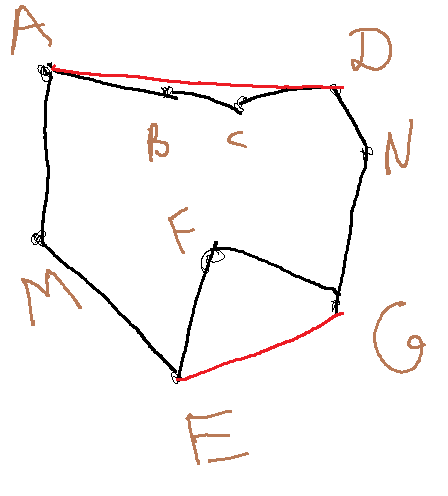
\includegraphics[scale=0.7]{1}\\
 	 в даном случае остается проверить для точки $U = (x, y), \; U \in ADGEM \cap U \notin FEG \cap U \notin ABCD$. \par
 	 Как же найти такие EFG? Как мы знаем уравнение прямой выглядит так: $\cfrac{x-x_1}{x_2 - x_1} = \cfrac{y-y_1}{y_2 -y_1}$. Теперь как определить что точка лежит справа? Можно просто посмоттеть где прямая через т U пересекает ось X например:\\
 	 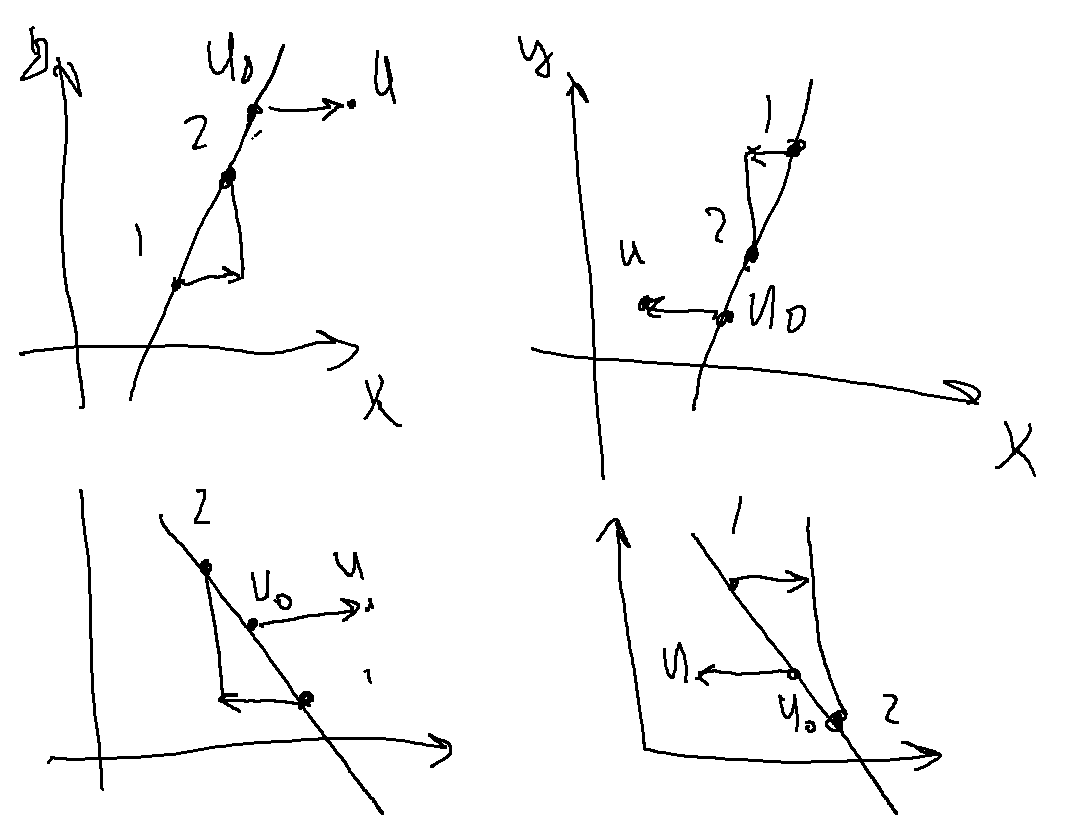
\includegraphics[scale=0.9]{2}\\
 	 \hspace*{1cm}Подставим y от U в уравнение получим:$x_3 =\cfrac{(y_U-y_1)(x_2 - x_1)}{y_2 -y_1} + x_1 $ тогда $U_0 = (x_3, y_U)$ тогда если $\cfrac{x_1 - x_2}{y_1 - y_2} > 0$ то U должна лежать правее точки $U_0$ получаем по знаку $x_U - \cfrac{(y_U-y_1)(x_2 - x_1)}{y_2 -y_1} - x_1\equiv x_2 - x_1$ иначе U должна лежать левее точки $U_0$ получаем по знак $x_U - \cfrac{(y_U-y_1)(x_2 - x_1)}{y_2 -y_1} - x_1\equiv -(x_2 - x_1)$ соеденяем получаем $x_U - \cfrac{(y_U-y_1)(x_2 - x_1)}{y_2 -y_1} - x_1\equiv \cfrac{x_1 - x_2}{y_1 - y_2}\cdot(x_2 - x_1)\implies (x_U -x_1) - \cfrac{(y_U-y_1)(x_2 - x_1)}{y_2 -y_1}\equiv \cfrac{(x_2 - x_1)^2}{y_2 - y_1}\implies(x_U -x_1)(y_2-y_1) - (y_U-y_1)(x_2 - x_1)\equiv (x_2 - x_1)^2 \implies(x_U -x_1)(y_2-y_1) - (y_U-y_1)(x_2 - x_1)\equiv1\implies(x_U -x_1)(y_2-y_1) > (y_U-y_1)(x_2 - x_1)$. Случай $U \in \cfrac{x-x_1}{x_2 - x_1} = \cfrac{y-y_1}{y_2 -y_1}$ нужно расмотреть отдельно но пусть в таком счучае будем считать, что принадлежит.
 	 \subsection{Итоговые Входные даные}
 	 Итак мы упрастили ввод до точек каждой из которой принадлежит ярлык ЦА или просто регион и какя то цифра хорактерезующая количество отправок.
 	 \section{Преобразование векторный графики в точечную}
 	 \subsection{Точка}
 	 \hspace*{1cm}Для начала хорошо бы создать класс точка с полями x, y. Так же прописать функцию поиска растояния и функции отрезка. Функцию отрезка можно получить вида $y=f(x)$ из ранее уже выведеной.
 	 \begin{verbatim}
 	 	import math
 	 	class point:
 	 	    def __init__(self, x:float, y:float):
 	 	        self.x = x
 	 	        self.y = y
 	 	
 	 	    def lenf(self, other):
 	 	        return math.sqrt((self.x - other.x)** 2 + (self.y - other.y)** 2)
 	 	
 	 	    def equatian(self, other, **printer):
 	 	        x_1, y_1 = self.x, self.y
 	 	        x_2, y_2 = other.x, other.y
 	 	        equatin = f"x * {(y_2 - y_1) / (x_2 - x_1)} - {x_1 * (y_2 - y_1) / (x_2 - x_1) + y_1}"
 	 	        if printer:
 	 	            print(f"y = {equatin}")
 	 	        return equatin
 	 	    
 	 	    def __hash__(self):
 	 	        return hash((self.x, self.y))
 	 \end{verbatim}
 	 И для красоты добавим функции print-а.
 	 \begin{verbatim}
 	 	    def __str__(self):
 	 	        return f"({self.x}, {self.y})"
 	 	    
 	 	    def __repr__(self):
 	 	        return f"<<{self.x}, {self.y}>>"
 	 \end{verbatim}
 	 \subsection{Лежит точка справа от отрезка?}
 	 \hspace*{1cm}Функция принисает 3 точки 2 из которых задают направленую прямую и 3-я это проверяемая точка. Все необходимые функции мы уже вывели.
 	 \begin{verbatim}
 	 	def point_right_line(point1, point2, u) -> bool:
 	 	    return (u.x - point1.x) * (point2.y - point1.y) > (u.y - point1.y) * (point2.x - point1.x)
 	 \end{verbatim}
 	 \subsection{Работа с выпуклой фигуры}
 	 \hspace*{1cm}Проверяем лежит ли точка в выпуклой фигуре. 
 	 \begin{verbatim}
 	 def point_in_normal_figure(pl:List[Point], u:Point):
 	     if len(pl) < 3: print("errore!!!!! Beckend  line")
 	     orintation_right = point_right_line(pl[0], pl[1], pl[2])
 	     point1 = pl[0]
 	     for point2 in pl[1:]:
 	         if orintation_right != point_right_line(point1, point2, u):
 	             return False
 	         point1 = point2
 	     if orintation_right != point_right_line(pl[-1], plt[0], u):
 	         return False
 	     return True
 	 
 	
 	 \end{verbatim}
 	 \subsection{Впуклый многоугольник}
 	 \hspace*{1cm}Самое сложное определить находится внутряняя часть фигуры справа или слева. Я предлагаю способ, который возможно будет работать не вегда, но в большинстве способов. Просто определить для каждого отрезка сколько точек лежит справа сколько слева. И так для всех и сложить. Получим два числа например r, l(r-спрва l-слева). И тогда если $r>l$ то спарава иначе слева. \par
 	 Тогда код будет выглядеть так:
 	 \begin{verbatim}
 	 def orintation_righ(main_fig:List[Point]):
 	     r, l = 0, 0
     	 temp_ln = len(main_fig)
 	     for i in range(temp_ln):
 	         for j in range(temp_ln):
 	             if j != i and j != (i + 1) % temp_ln:
 	                 if point_right_line(main_fig[i], main_fig[(i + 1) % temp_ln], main_fig[j]):
 	                 r += 1
 	             else:
 	                 l += 1
 	     return r > l
 	 
 	 
 	 
 	 def point_in_bad_figure(main_fig:List[Point], u:Point):
 	     added_fig = []
 	     orintation_right = orintation_righ(main_fig)
 	     count = 0
 	     i = 0
 	     while True:
 	         points = [main_fig[i], main_fig[(i + 2)% len(main_fig)], main_fig[(i + 1)% len(main_fig)]]
 	         if (point_right_line(points[0], points[1], points[2]) and (not orintation_right)) or ((not point_right_line(points[0], points[1], points[2])) and orintation_right):
 	             count += 1
 	         else:
 	             added_fig += [points]
 	             main_fig.remove(main_fig[(i + 1)% len(main_fig)])
 	             count = 0
 	         i += 1
 	         if count + 3 == len(main_fig):     
 	             break
 	     in_fig = point_in_normal_figure(main_fig, u)
 	     for i in added_fig:
 	         in_fig = infig and not point_in_normal_figure(i, u)
 	     return in_fig
 	\end{verbatim}
 	\section{Алгоритм}
 	\subsection{Функция точки}
 	\hspace*{1cm}Опредлим эту функцию из логики того, что на нее влияет. Итак она будет зависить от населености района, где она стоит и от ближайших ЦА. Пусть $peple(x,y)$ это население в точки x, y, $Bcentr(x,y)$ вернет роходимость Бизнес центра в точке x, y, если там нет бизнес центра вернет 0, $Tcenter(x, y), storegge(x,y)$ аналогично для торогого цента и склада. Получаем что то типо:
 	\[f(x, y)= \bigg(\sum_{-R_1<i<R_1}\sum_{-R_1<j<R_1}\cfrac{k_1}{\sqrt{i^2 + j^2}^2}\cdot peple(i,j)\bigg) +\bigg( \sum_{-R_2<i<R_2}\sum_{-R_2<j<R_2}\cfrac{k_2}{\sqrt{i^2 + j^2}^3} \cdot Bcentr(i,j) \bigg)+ \]
 	\[+\bigg( \sum_{-R_2<i<R_2}\sum_{-R_2<j<R_2}\cfrac{k_3}{\sqrt{i^2 + j^2}^3} \cdot Tcenter(i,j) \bigg) + \bigg( \sum_{-R_2<i<R_2}\sum_{-R_2<j<R_2}\cfrac{k_4}{\sqrt{i^2 + j^2}^3} \cdot storegge(i,j) \bigg)\] 
 	\par $R_1, R_2$ мы договорились взять 1 km и 500m, а $k_1, k_2, k_3,k_4$ зависят от входных данных, они будут определны дополнительными расчетами и R определим позже. 
    \hspace*{1cm}Теперь осталось дописать систему поиска точки с наибольшем значением функции и не забыть про влияние поставленных почтаматов на ставящийся.
    \section{ссылки}\label{Referenses}
 \end{document}